\documentclass{beamer}

%lembre-se de configurar o pdflatex com:
%pdflatex -shell-escape -synctex=1 -interaction=nonstopmode  -output-directory=build  %.tex

\usepackage{aula}
\usetikzlibrary{shapes.geometric, positioning}
\title{Contêineres}
\date{\today}

\begin{document}
    
\input{capa}

\section{Conceitos de containerização}
\begin{frame}{Docker: Conceito geral}
    
    \textbf{Docker} é uma plataforma para executar aplicações em \textbf{containers}.
    
    \vspace{0.4cm}
    
    \textbf{Container:}
    
    \begin{itemize}
        \item Ambiente isolado
        \item Inclui aplicação + dependências
        \item Executa sobre o \textit{kernel} do sistema operacional (geralmente Linux)
    \end{itemize}
    
    \vspace{0.4cm}
    
    \textbf{Vantagens:}
    
    \begin{itemize}
        \item Reprodutibilidade de ambientes
        \item Portabilidade entre máquinas
        \item Facilidade de distribuição de software
        \item Muito usado em \textit{deploy} e ciência de dados
    \end{itemize}
    
\end{frame}

\begin{frame}[fragile]{Docker: Instalação no Windows}
    
    No Windows, Docker é instalado através do \textbf{Docker Desktop}.
    
    \vspace{0.3cm}
    \textbf{1. Instalar o subsistema Linux do Windows (WSL)}
    \begin{minted}{powershell}
wsl --install
    \end{minted}   
    
    \textbf{2. Instalar o Docker via Winget}
    
    \begin{minted}{powershell}
winget install Docker.DockerDesktop
    \end{minted}
    
    \textbf{3. Reiniciar o computador}
    
    \textbf{4. Verificar instalação}
    
    \begin{minted}{bash}
docker --version
docker run hello-world
    \end{minted}
    
    \textbf{Requisitos}
    
    \begin{itemize}
        \item Windows 10 ou 11
        \item Virtualização habilitada
        \item WSL2 instalado
    \end{itemize}
    
\end{frame}

\begin{frame}{Docker: Arquitetura}
    
    \begin{center}
        
        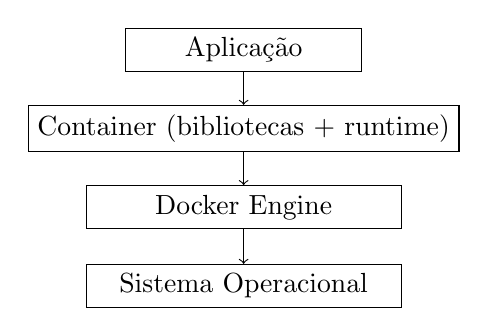
\begin{tikzpicture}[node distance=1cm]
            
            \node[draw, rectangle, minimum width=3cm] (app) {Aplicação};
            
            \node[draw, rectangle, minimum width=4cm, below of=app] (container)
            {Container  (bibliotecas + runtime)};
            
            \node[draw, rectangle, minimum width=4cm, below of=container] (engine)
            {Docker Engine};
            
            \node[draw, rectangle, minimum width=4cm, below of=engine] (os)
            {Sistema Operacional};
            
            \draw[->] (app) -- (container);
            \draw[->] (container) -- (engine);
            \draw[->] (engine) -- (os);
            
        \end{tikzpicture}
        
    \end{center}
    
    Componentes principais:
    
    \begin{itemize}
        \item \textbf{Docker Engine} — executa containers
        \item \textbf{Images} — modelos de containers (receitas de bolo)
        \item \textbf{Containers} — instâncias executáveis das imagens (bolo)
    \end{itemize}
    
\end{frame}

\begin{frame}[fragile]{Docker: Conceitos principais}
    
    \textbf{Imagem (Image)}
    
    \begin{itemize}
        \item Modelo imutável de um container
        \item Contém sistema base + dependências
    \end{itemize}
    
    \textbf{Container}
    
    \begin{itemize}
        \item Instância em execução de uma imagem
    \end{itemize}
    
    \textbf{Exemplo de execução}
    
    \begin{minted}{bash}
docker run hello-world
    \end{minted}
    
    Fluxo típico:
    
    \begin{enumerate}
        \item baixar a imagem
        \item criar um container
        \item executar a aplicação
    \end{enumerate}
    
\end{frame}

\begin{frame}[fragile]{Docker: Dockerfile — criando imagens}
    
    Um \textbf{Dockerfile} descreve como construir uma imagem.
    
    Exemplo simples:
    
    \begin{minted}{dockerfile}
FROM python:3.11

WORKDIR /app

COPY app.py .

RUN pip install numpy

CMD ["python", "app.py"]
    \end{minted}
    
    Construção da imagem:
    
    \begin{minted}{bash}
docker build -t meu_app .
    \end{minted}
    
    Execução:
    
    \begin{minted}{bash}
docker run meu_app
    \end{minted}
    
\end{frame}

\begin{frame}{Docker vs Máquina Virtual}
    
    \begin{center}
        
        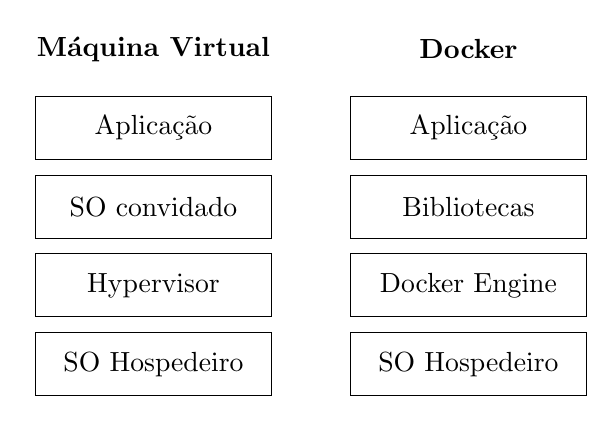
\begin{tikzpicture}[
            node distance=1cm,
            box/.style={draw, rectangle, minimum width=3cm, minimum height=0.8cm}
            ]
            
            % títulos
            \node (title1) {\textbf{Máquina Virtual}};
            \node[right of=title1, xshift=3cm] (title2) {\textbf{Docker}};
            
            % coluna VM
            \node[box, below of=title1] (vmapp) {Aplicação};
            \node[box, below of=vmapp] (vmos) {SO convidado};
            \node[box, below of=vmos] (hyper) {Hypervisor};
            \node[box, below of=hyper] (host) {SO Hospedeiro};
            
            % coluna Docker
            \node[box, below of=title2] (dapp) {Aplicação};
            \node[box, below of=dapp] (dlib) {Bibliotecas};
            \node[box, below of=dlib] (engine) {Docker Engine};
            \node[box, below of=engine] (host2) {SO Hospedeiro};
            
        \end{tikzpicture}
        
    \end{center}
    
    \begin{itemize}
        \item VM inclui um \textbf{sistema operacional completo}
        \item Containers compartilham o \textbf{kernel do host}
        \item Containers são mais \textbf{leves e rápidos}
    \end{itemize}
    
\end{frame}

\begin{frame}{Tipos de hospedagem para sistemas web}

\begin{figure}
\centering
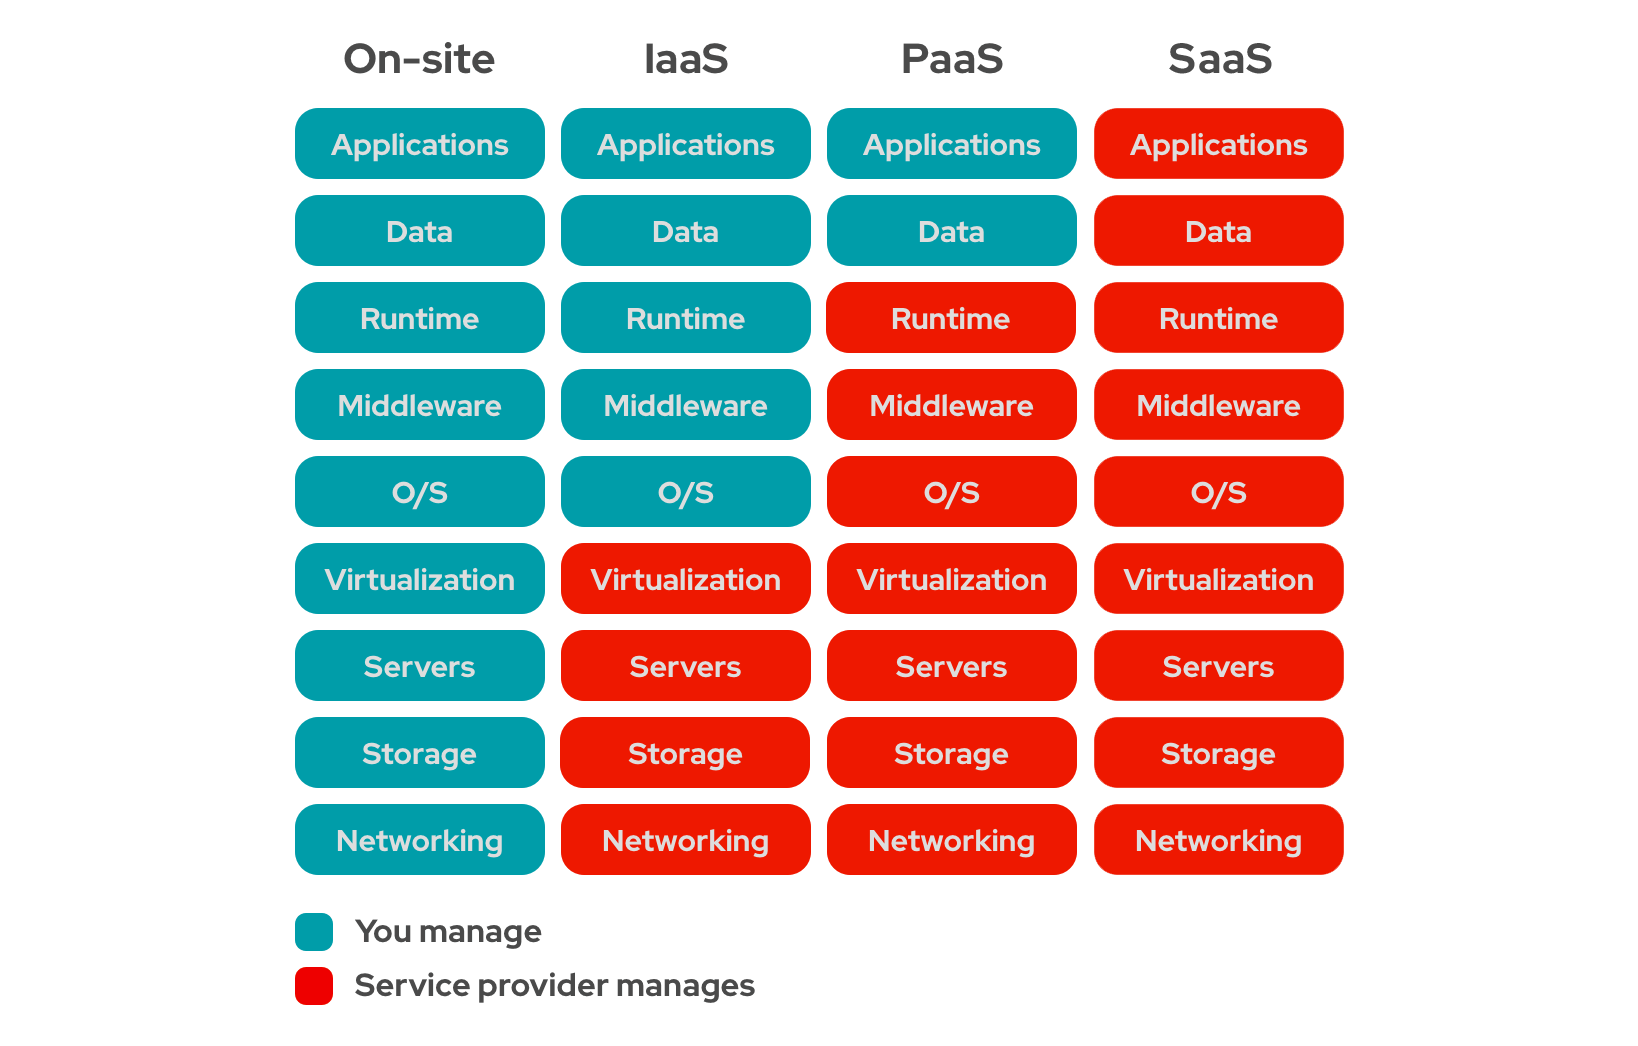
\includegraphics[width=0.7\linewidth]{bancos_de_dados_relacionais_figs/iaas-paas-saas-diagram5.1-1638x1046}
\caption{Quero hospedar meu site. O que um datacenter pode me oferecer? Fonte: \url{https://www.redhat.com/pt-br/topics/cloud-computing/iaas-vs-paas-vs-saas}}
\end{figure}

\end{frame}

\begin{frame}[fragile]{Docker Volumes — Persistência de dados}
    
    Containers são \textbf{efêmeros}: quando removidos, os dados internos são perdidos.
    
    \vspace{0.3cm}
    
    \textbf{Docker Volumes} permitem armazenar dados fora do container.
    
    \begin{center}
        
        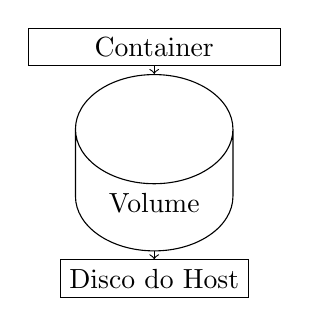
\begin{tikzpicture}[node distance=0.1cm]
            
            \node[draw, rectangle, minimum width=3.2cm] (container) {Container};
            
            \node[
                draw,
                cylinder,
                shape border rotate=90,
                minimum height=0.2cm,
                minimum width=2cm,
                below=of container
            ] (volume) {Volume};
            
            \node[
                draw,
                rectangle,
                minimum width=1.2cm,
                below=of volume
            ] (host) {Disco do Host};
            
            \draw[->] (container) -- (volume);
            \draw[->] (volume) -- (host);
            
        \end{tikzpicture}
        
    \end{center}

    
    \textbf{O volume pode ser uma pasta passada na hora da criação do container (-v).}
    
    \textbf{Vantagem}
    
    \begin{itemize}
        \item Dados persistem mesmo se o container for removido
    \end{itemize}
    
\end{frame}

\begin{frame}[fragile]{PostGIS em Docker}
    
    Um banco espacial pode ser iniciado rapidamente com Docker.
    
    \vspace{0.3cm}
    
    Baixar, criar e executar um container PostGIS:
    
    \begin{minted}{bash}
docker run -d \
-p 5432:5432 \
-e POSTGRES_PASSWORD=postgres \
--name postgis \
-v dados_postgres:/var/lib/postgresql/data \
postgis/postgis
    \end{minted}
    
    Agora o banco pode ser acessado com:
    \begin{minted}{bash}
docker exec -it postgis psql -U postgres
    \end{minted}
    ou
    \begin{itemize}
        \item QGIS
        \item DBeaver
        \item Python (psycopg)
    \end{itemize}
    

    
\end{frame}

\section{PostgreSQL+PostGIS em Docker}

\begin{frame}[fragile]{PostGIS em Docker}
    A imagem postgis/postgis já carrega a extensão espacial PostGIS e todos bancos de dados criados. 
    \vspace{0.3cm}

    Teste se o postgis estáinstalado no banco. (acessar o banco usando psql)
    
    \begin{minted}{sql}
SELECT PostGIS_Version();
    \end{minted}

    Não é necessário executar o comando: 
    \begin{minted}{sql}
CREATE EXTENSION PostGIS;
    \end{minted}

\end{frame}

\begin{frame}[fragile]{Comandos úteis do Docker}
    
    \textbf{Listar containers}
    
    \begin{minted}{bash}
docker ps          # containers em execução
docker ps -a       # todos os containers
    \end{minted}
    
    \textbf{Parar um container}
    
    \begin{minted}{bash}
docker stop <container_id>
    \end{minted}
    
    \textbf{Iniciar um container parado}
    
    \begin{minted}{bash}
docker start <container_id>
    \end{minted}
    
    \textbf{Remover um container}
    
    \begin{minted}{bash}
docker container rm <container_id>
    \end{minted}
    
    \textbf{Exemplo de fluxo típico}
    
    \begin{minted}{bash}
docker run -d postgis/postgis --name postgis
docker ps
docker stop postgis
docker start postgis
docker container rm postgis
    \end{minted}
    
\end{frame}

\begin{frame}{Cheat sheet}
\centering 
Lista de comandos docker úteis (mas você pode fazer pelo Desktop).
\large \url{https://docs.docker.com/get-started/docker_cheatsheet.pdf}
\end{frame}

\section{PostgreSQL+PostGIS com Docker compose}

\begin{frame}[fragile]{Docker Compose: Conceitos}

\textbf{Docker Compose} permite definir e executar múltiplos containers usando um único arquivo YAML.

\vspace{0.4cm}

\textbf{Principais conceitos:}

\begin{itemize}
    \item \textbf{services}
    \begin{itemize}
        \item Containers da aplicação
    \end{itemize}

    \item \textbf{image}
    \begin{itemize}
        \item Imagem Docker utilizada
    \end{itemize}

    \item \textbf{ports}
    \begin{itemize}
        \item Mapeamento de portas
    \end{itemize}

    \item \textbf{volumes}
    \begin{itemize}
        \item Persistência de dados
    \end{itemize}

    \item \textbf{environment}
    \begin{itemize}
        \item Variáveis de ambiente
    \end{itemize}
\end{itemize}

\vspace{0.4cm}

\textbf{Execução:}

\begin{minted}{bash}
docker compose up -d
\end{minted}

\end{frame}

\begin{frame}[fragile]{Exemplo: PostGIS com Docker Compose}
Salvar em \textbf{docker-compose.ym}l e executar \textbf{ docker compose up} .
\begin{minted}{yaml}
version: '3.9'

services: # Todos os containers serao descritos aqui
  postgis: # Nome do container no compose
    image: postgis/postgis # Imagem a ser utilizada: PostgreSQL + PostGIS
    container_name: postgis # Nome do container
    restart: unless-stopped # Reinício automático do serviço

    ports:
      - "5432:5432" # Porta local 5432 → container 5432

    environment: # Variáveis de ambiente
      POSTGRES_PASSWORD: postgres

    volumes:  # Ligações entre pastas do hospedeiro e do container.
      - dados_postgres:/var/lib/postgresql/data

volumes: # Lista de volumes. Vários containers podem usar os mesmos volumes.
  dados_postgres: # Volume mantém os dados persistentes
\end{minted}

\vspace{0.3cm}

\end{frame}

\end{document}
